
Completed reductions can be 'Archived' (i.e. declared 'completed'
because no more work is needed) and removed from the Reduction
Queue. Additionaly, even if all products for all tasks are saved in
the EDPS\_data directory, the most important producs can be
`exported' to a desired location.

To do so, proceed as follows:

\begin{enumerate}
\item In the `Reduction Queue` tab, select the dataset and the dataset
  for which you want to export the final products, and press the
  'Archive' button.
  
\begin{figure}[h!]
\centering
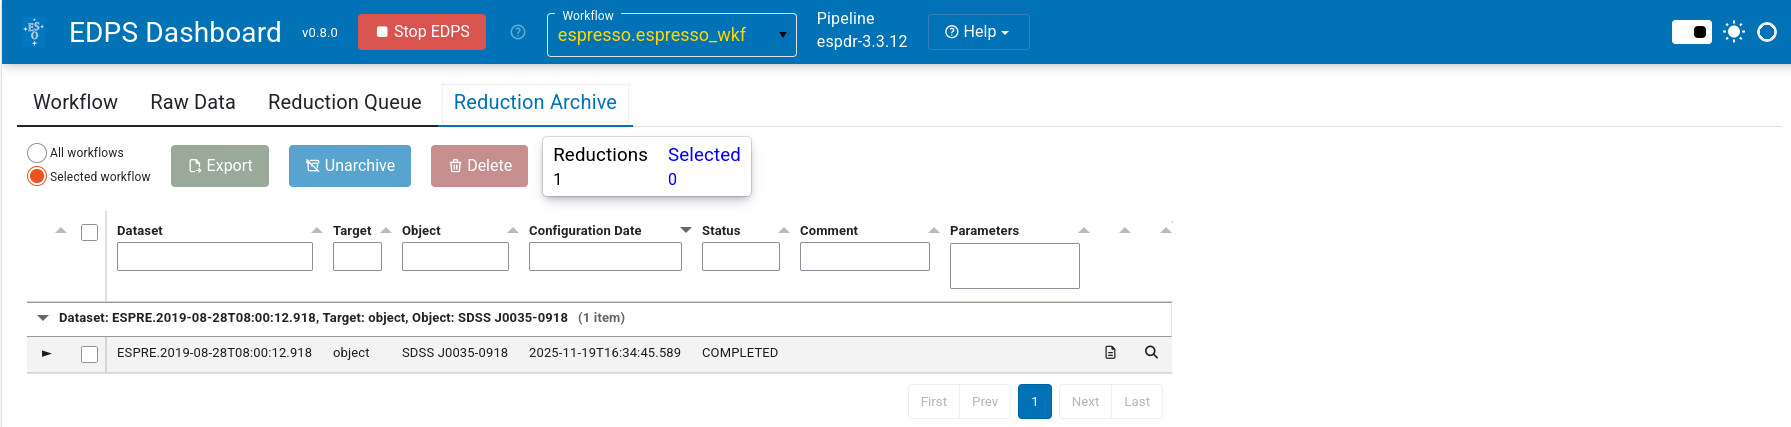
\includegraphics[width=0.8\textwidth]{../instrument_tutorial/figures/archive.jpg}
\caption{How to archive a completed reduction from the Reduction Queue tab.}
\end{figure}



\item Go in the Reduction Archive tab and click on the 'Export'
  button. A new tab window appear where you can indicate the directory
  you want to copy your final products; finally press "Export" to copy
  the data.


\begin{figure}[h!]
\centering

\includegraphics[width=0.8\textwidth]{../instrument_tutorial/figures/export1.jpg}
\caption{The reduction archive tab. This table contains all the different configurations of datasets that are declared "finished" and removed from the Reduction Queue. From this page, the user can export the most important files into a desired local directory.}
\end{figure}



\begin{figure}[h!]
\centering

\includegraphics[width=0.7\textwidth]{../instrument_tutorial/figures/export2.jpg}
\caption{The EXPORT dialogue window, where the user can decide which reduced configuration to save and where.}
\end{figure}

\end{enumerate}
